\paragraph{Quality Control.} Genotyping was carried out at the Genotyping and Microarray facility at the Wellcome Trust Sanger Institute, UK  and Duke-NUS Medical School, Singapore. Genotypes were assessed in five batches using Illumina HumanOmniExpress- 12v1-1 (; Sanger, two batches), Illumina HumanOmniExpress- 24v1-0 (Duke-NUS, two batches) and Illumina HumanOmniExpress- 24v1-1 chips (Duke-NUS). An overview of probe-overlap between the batches is depicted in Figure~\ref{fig:probeoverlap}. Probes targeting the same SNP on the different chip versions were confirmed to have the same sequence. SNPs were called via the GenCall software for clustering, calling and scoring of genotypes \citep{Teo2007}. For batches run on the same platform, genotype signals were combined and called in a single analysis, leading to three independent genotype batches for quality control (QC) and imputation: sanger12 (1,344 samples), Duke-NUS12 (284 samples), Duke-NUS3 (96 samples).

Prior to QC, rsID descriptions (chromosome, chromosomal positions and allele order) of the three batches were matched to the reference set used for imputation (combined UK10K and 1000 Genomes reference panel) and ensembl human variation annotation (GRCh37p13, 15.04.2016) for rsIDs not included in the reference panel. rsIDs that matched to neither referenc were removed from further analyses. The quality of the genotypes was evaluated both on a per-individual and per-marker level following an adapted quality control protocol of Anderson and colleagues \citep{Anderson2010}. Unless stated otherwise, the PLINK software (version 1.9) \citep{Purcell2007, Chang2015} was used for all QC analyses. In summary, the per-individual QC included the identification of individuals with discordant sex information, missing SNP rates (more than 3\% of SNPs not called) and outlying heterozygosity rates (outside 3 standard deviations of mean heterozygosity rate). Population substructures arising due to different ethnical origins of samples were examined by comparison of sample genotypes to genotypes of the HapMap Phase III study \citep{HapMap2005} from four ethnic populations. Samples that clustered with HapMap III individuals of caucasian ancestry were kept for further analyses (Figure~\ref{fig:pca}). The per-marker QC included filtering of SNPs with missing call rate in more than 1\% of the samples and SNPs which significantly deviate from Hardy-Weinberg equilibrium (HWE, p < 0.001). The number of samples and SNPs excluded at each QC step are summarised in Table~\ref{tab:genoQC}. Table~\ref{tab:genoOverview} shows an overview of sample and SNP numbers before and after the QC described above. 

\begin{figure}[!tbp]
	\centering
	\begin{subfigure}[b]{0.3\textwidth}
		\center
		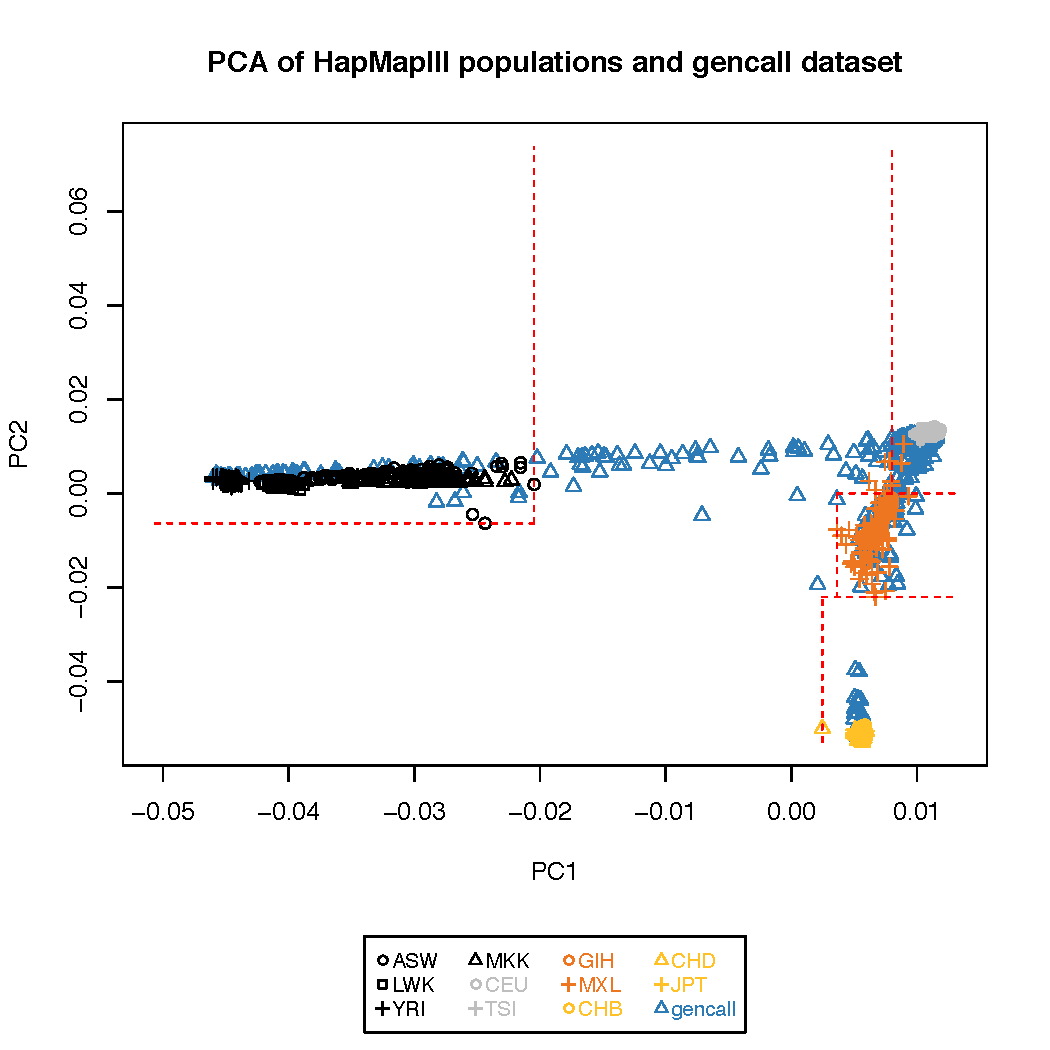
\includegraphics[trim = 0mm 0mm 10mm 25mm, clip,scale=0.3,page=1]{FiguresTablesGenotypes/pca_overview_sanger12_singapore123.pdf}	
		\caption{\textbf{Sanger12}}
		\label{fig:pca1}	
	\end{subfigure}
	~
	\begin{subfigure}[b]{0.3\textwidth}
		\center
		\includegraphics[trim = 0mm 0mm 10mm 25mm, clip,scale=0.3, page=2]{FiguresTablesGenotypes/pca_overview_sanger12_singapore123.pdf}	
		\caption{\textbf{Duke-NUS12}}
		\label{fig:pca1}	
	\end{subfigure}
	~
	\begin{subfigure}[b]{0.3\textwidth}
		\center
		\includegraphics[trim = 0mm 0mm 10mm 25mm, clip,scale=0.3, page=3]{FiguresTablesGenotypes/pca_overview_sanger12_singapore123.pdf}	
		\caption{\textbf{Duke-NUS3}}
		\label{fig:pca1}	
	\end{subfigure}
  \caption{\textbf{Principal Component Analysis of the three genotype sets with HapMapIII genotypes.} }
   	\label{fig:pca}
\end{figure}




% Table generated by Excel2LaTeX from sheet 'GenotypesSummaryHVOL'
\begin{table}[htbp]
  \centering
  \caption{\textbf{Overview of genotype data before and after quality control.}}
    \begin{tabular}{llrllrr}
    		\toprule
          & \multicolumn{2}{c}{\textbf{pre-QC}} &  &\multicolumn{3}{c}{\textbf{post-QC}} \\
          \cmidrule{2-3}\cmidrule{5-7}
          & samples (m/f) & \multicolumn{1}{l}{SNPs} & & samples (m/f) & \multicolumn{1}{l}{SNPs} & \multicolumn{1}{l}{genotyping rate} \\
            \cmidrule{2-7}
    \textbf{Sanger12} & 1344  (614/  730) & 719,665 & & 998 (463/535) & 677,036 & 0.997678 \\
    \textbf{Duke\_NUS12} & 284 (118/ 166) & 716,503 &  &179 (68/ 111) & 682,016 & 0.998253 \\
    \textbf{Duke-NUS3} & 96 (48/ 48) & 713,014 &  &62 (34/ 28) & 657,497 & 0.997916 \\
    \bottomrule
    \end{tabular}%
  \label{tab:genoOverview}%
\end{table}%


\paragraph{Phasing and Imputation.} Phasing and imputation were conducted in two separate steps. The SHAPEIT software (version 2) \citep{Delaneau2012,Delaneau2013} was used to generate a set of estimated haplotypes based on the combined 1000 Genomes \citep{Abecasis2012} and UK10K \citep{UK10KConsortium2014} reference panel as genetic map. The same reference panel was used for the imputation of the samples’ genome-wide SNP genotypes via the IMPUTE2 software (version 2.3.0) \citep{Marchini2007, Howie2009}. 
\paragraph{Combining dataset}. The three genotype batches were combined after imputation and filtered again on a per-marker and per-sample level. SNPs with a certainty score of less than 0.4 in at least one of the batches were excluded from further analyses. None of the xxx SNPs had to be removed due to significant differential missingness (p < 1e-5) across the three batches. After combining the three datasets, SNPs were filtered for deviation from HWE (p <0.001) and a minor allele count of at least 20 alleles (corresponding to a minor allele frequency of xxx).  On sample level, related individuals were excluded from the dataset in order to remove bias towards genotypes shared within a family and to accurately represent the allele frequency of the entire population. Relatedness was estimated by the proportion of SNPs shared between two individuals and subsequent calculation of identity by descent estimated as PI\_HAT via PLINK as described in \citep{Anderson2010}. From any pair of individuals with a PI\_HAT of greater than 0.125 , the individual with the higher SNP calling rate was retained in the analysis. 

After imputation and imputation quality control, the data set contains xxx SNPs. IMPUTE2 yields imputed genotypes encoded in triplets of posterior probabilities for the possible allele combinations \((AA, AB, BB)\). These genotypes were converted into an expected genotype \(G\) by the dosage model \citep{Howie2011}:

\begin{equation}
	G = 0 \times p(AA) + 1 \times p(AB) + 2 \times p(BB) = p(AB) + 2 \times p(BB)
\end{equation}


